% USE PDFLatex!
% to correctly render Swedish characters
% From: https://bitbucket.org/flavius_gruian/msccls/src/master/popsci/popsci.tex

\documentclass{popsci}

\usepackage[utf8]{inputenc}
\usepackage[swedish, english]{babel}

\usepackage{fancyhdr}
\usepackage{titling}
\usepackage{color}
\usepackage{colortbl}
\usepackage{graphicx}
\usepackage{flushend}
\usepackage{lmodern}
\usepackage{lipsum}  


% Please specify the presentation date
\presentationsdag{2021-10-28}

% use either of these commands to specify the title of your thesis
%\examensarbete{Klassificering av hjärnaktivitet med elektroencephalografi och automatiserad tidsspårning av datoranvändning}
% To create a title in two rows, leave examensarbete blank and fill in examensarbeteTwoRows.
\examensarbeteTwoRows{Classifying brain activity using electroencephalography and automated time}{tracking of computer use}
\student{Erik Bjäreholt}
\supervisor{Markus Borg (LTH / RISE)}
\examiner{Elizabeth Bjarnarson (LTH)}

% Your pop-sci title should be different (more catchy) than your thesis title
\title{Hur kan man läsa programmerares tankar?}

\begin{document}

% not more than 4 rows!
\theabstract{Kan man läsa tankar? Kanske inte, men genom att mäta hjärnaktivitet går det att skilja mellan olika datoraktiviteter. Så även om man inte kan läsa tankar, så kan man iallafall urskilja vad man tänker på, given ett par alternativ.} % Till exempel är det möjligt att veta om en programmerare läser kod eller vanlig text. 

% När man skriver sammanfattningen är det viktigaste att skriva enkelt och begripligt. Den som inte alls är insatt i ämnet ska kunna förstå vad ditt arbete handlar om. Förklara vad du kommit fram till och, om det går, vad forskningen kan användas till.  Sammanfattning bör vara mellan 1500 och 4000 tecken. 

\noindent Vi har studerat om man kan använda billig neuroteknik (under 10,000kr) för att urskilja vad en person gör på datorn. I synnerhet om en person läser text eller kod.

Vi har använt EEG, eller elektroencefalografi som det heter, vilket är en teknik som mäter hjärnaktivitet med hjälp av elektroder som sätts på huvudet. Elektroderna mäter små spänningsskillnader över hjärnan som skapas när hjärnceller aktiveras. Dessa mätningar sker 256 gånger per sekund och bildar en EEG-signal som informellt kallas ``hjärnvågor''. Denna signal kan man sedan applicera olika tekniker och maskininlärningsmetoder på för att detektera vissa typer av hjärnaktivitet.

%\begin{figure}[!bth] % Use pictures in your pop-vet!
%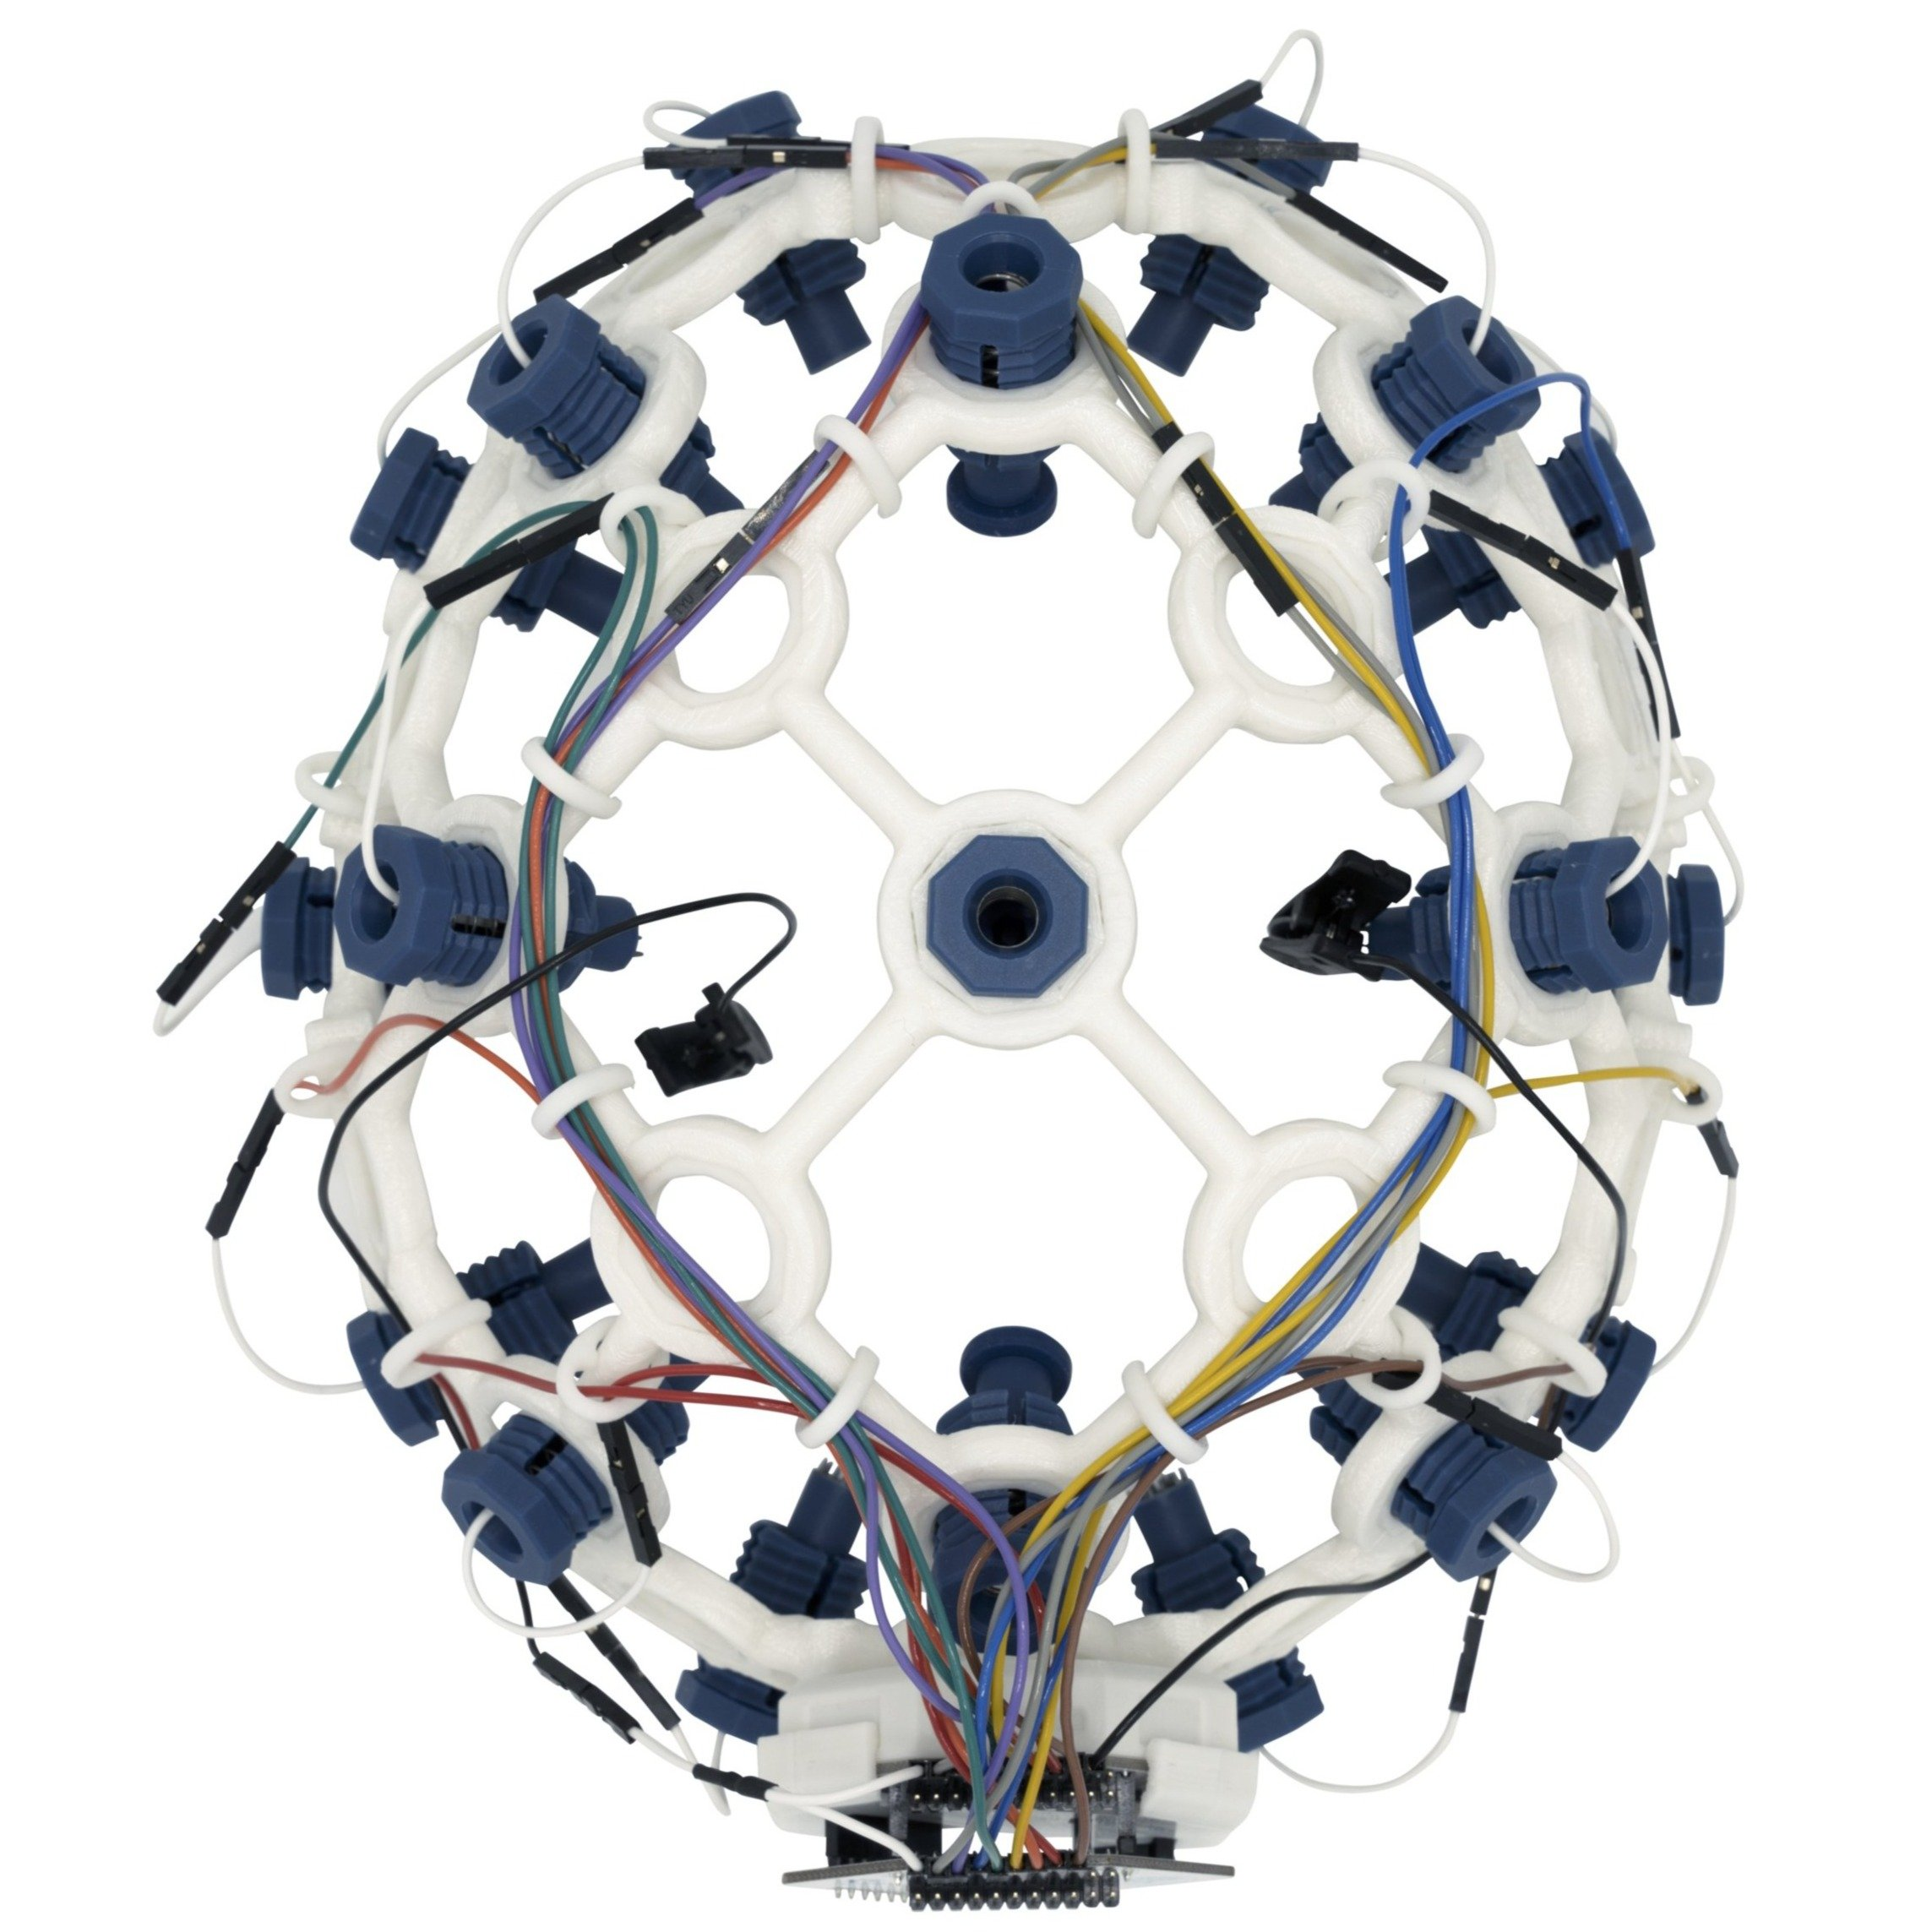
\includegraphics[angle=90, trim=200 50 250 100,clip, width=\columnwidth]{img/openbci-cyton.jpg} 
%    \caption{Ett 3D-printat EEG headset (OpenBCI Ultracortex Mark IV) kopplat med EEG-enheten OpenBCI Cyton.}
%\end{figure}

% Hur gjorde du?
Vi använde en billig EEG enhet (ca 3000kr) för att mäta 9 utvecklares ``hjärnvågor'' under olika datoraktiviteter. I synnerhet medans de antingen läser ett kodproblem, eller granskar en bit prosa. Vi använde sedan maskininlärningsmetoder för att lära en algoritm urskilja de två aktiviteterna med hjälp utav bara EEG-signalen.

Utöver vårat ``kod eller prosa'' experiment utförde vi även ett experiment i en naturlig miljö, där en utvecklare fritt fick använda sin dator till olika aktiviteter. Med hjälp av vårat tidigare utvecklade program ActivityWatch, som automatiskt spårar hur man spenderar sin tid vid datorn, kan vi då märka upp tidsintervallen när personen skrev kod, skrev prosa, scrollade på Twitter, eller tittade på YouTube. 

Vi tränade sedan igen maskininlärningsalgoritmer för dessa 4 kategorier, och våra resultat visade att det gick bra att urskilja på aktiviteter som var arbete och inte arbete, medans det var svårare att urskilja olika arbets- eller rekreationsaktiviteter från varandra.

% Vad har du kommit fram till?
% Vi har kommit fram till att teknik såsom elektroencefalografi kan användas för att urskilja om en person läser kod eller prosa. Vi visar också att flera andra datoraktiviteter kan urskiljas med samma teknik.

% Hur påverkar dina rön människa och samhälle?
% Våran upptäckt kan hjälpa mjukvaruutvecklare att bättre kan förstå vad som händer i sin hjärna under sitt arbete.

% På vilket sätt kan resultaten användas?
% Det kan användas för att i realtid uppskatta om en mjukvaruutvecklare tänker på kod eller prosa. Möjligtvis som ett alternativt mått för fokus, dvs att inte bara mäta ifall personen är fokuserad, utan även hur fokuserad hen är på en specifik uppgift.
% Våran klassificering av om en programmerare tänker på kod eller prosa kan användas för att mäta utvecklarens fokus på just kod (och inte bara fokus generellt).

% Varför är ditt arbete viktigt?
Vårat arbete förbättrar tidigare studiers resultat för att urskilja om en utvecklare resonerar kring kod eller prosa. Utöver det är en del av studien den första av sin typ då den använder automatiserad tidsspårning av vad man gör vid datorn för att se ifall man kan klassificera flera olika datoraktiviteter i en naturlig miljö. Vi har även bidragit till utvecklingen av flera programvarubibliotek som används för denna typen av studier.

\end{document}
